\documentclass{article}

\usepackage{CJK}
\usepackage{graphicx}
\usepackage{amsmath}
\usepackage{color}
\usepackage{authblk}

\usepackage{geometry}
\usepackage{titlesec}


\addtolength{\topmargin}{-20pt}
\setlength{\oddsidemargin}{0.63cm}  % 3.17cm - 1 inch
\setlength{\evensidemargin}{\oddsidemargin}
\setlength{\textwidth}{14.66cm}
\setlength{\textheight}{22.00cm}    % 24.62

\linespread{1.5}
% \setlength{\parskip}{1ex}
\setlength{\parskip}{1\baselineskip}


\begin{document}


\title{\textbf{High-order Boltzmann Machine \\for Frame Ratio Upconversion}}
\author{Mingmin Zhao}
\affil{Department of Computer Science, Peking University, China}
%\author[*]{Author A}
%\author[*]{Author B}
%\author[*]{Author C}
%\author[**]{Author D}
%\author[**]{Author E}
%\affil[*]{Department of Computer Science, \LaTeX\ University}
%\affil[**]{Department of Mechanical Engineering, \LaTeX\ University}

\date{\today}
\maketitle
%\tableofcontents

%\newpage

\section{The binary-valued model}

\subsection{High-order Boltzmann Machine}

\begin{figure}
  \centering
  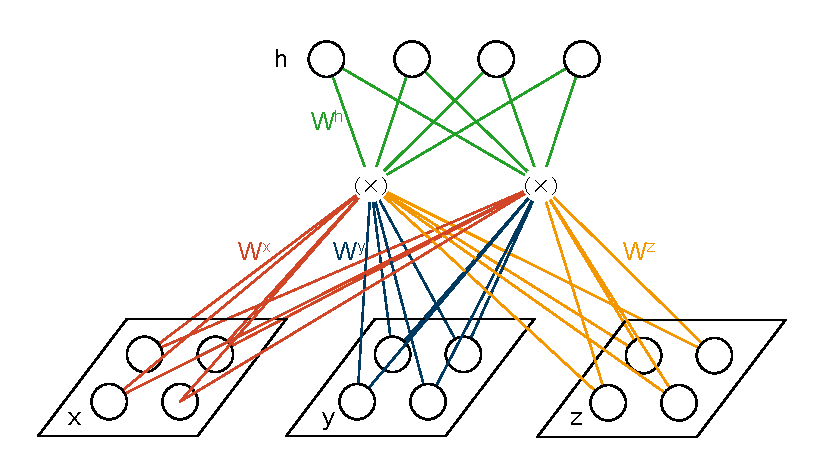
\includegraphics[width=4in]{4GRBM}\\
  \caption{Graphical representation of a 4-way gated Boltzmann machine}\label{4GRBM}
\end{figure}

A \textit{4-way gated Boltzmann machine} consists of $L$ hidden units $\boldsymbol{H} = (H_1, ..., H_L)$ to capture dependencies between three layers of observed variable with units $\boldsymbol{X} = (X_1, ..., X_I)$, $\boldsymbol{Y} = (Y_1, ..., Y_J)$ and $\boldsymbol{Z} = (Z_1, ..., Z_K)$.
The energy function of the model is defined as:
\begin{equation}
\begin{split}
E(\boldsymbol{x},\boldsymbol{y},\boldsymbol{z},\boldsymbol{h};\boldsymbol{\theta}) = &-\sum_f{\bigg(\sum_i{x_i w_{if}^x}\bigg) \bigg(\sum_j{y_i w_{jf}^y}\bigg) \bigg(\sum_k{z_k w_{kf}^z}\bigg) \bigg(\sum_l{h_l w_{lf}^h}\bigg)}
\\
&- \sum_i{w_{i}^x x_i} - \sum_j{w_{j}^y y_i} - \sum_k{w_{k}^z z_k} - \sum_l{w_{l}^h h_l}
\end{split}
\end{equation}

where $\boldsymbol{\theta} = \{\boldsymbol{W^x}, \boldsymbol{W^y}, \boldsymbol{W^z}, \boldsymbol{W^h}\}$ are the parameters of the model and each factor $f$ corresponds to a quadruplet of linear filters.

The joint probability distribution under the model is given by the Gibbs distribution:
\begin{equation}
p(\boldsymbol{x},\boldsymbol{y},\boldsymbol{z},\boldsymbol{h};\boldsymbol{\theta}) = \frac{1}{Z(\boldsymbol{\theta})}e^{-E(\boldsymbol{x},\boldsymbol{y},\boldsymbol{z},\boldsymbol{h};\boldsymbol{\theta})}
\end{equation}
where the \textit{partition} function $Z(\boldsymbol{\theta})$ is defined as:
\begin{equation}
Z(\boldsymbol{\theta}) = \sum_{\boldsymbol{x},\boldsymbol{y},\boldsymbol{z},\boldsymbol{h}}{e^{-E(\boldsymbol{x},\boldsymbol{y},\boldsymbol{z},\boldsymbol{h};\boldsymbol{\theta})}}
\end{equation}


\subsection{Conditionals}

\begin{equation}
p(x_i=1|\boldsymbol{y},\boldsymbol{z},\boldsymbol{h}) = \sigma[-\sum_f{ w_{if}^x (\sum_j{y_i w_{jf}^y}) (\sum_k{z_k w_{kf}^z}) (\sum_l{h_l w_{lf}^h})} - w_i^x]
\end{equation}

\begin{equation}
p(y_j=1|\boldsymbol{x},\boldsymbol{z},\boldsymbol{h}) = \sigma[-\sum_f{ w_{jf}^y (\sum_i{x_i w_{if}^x}) (\sum_k{z_k w_{kf}^z}) (\sum_l{h_l w_{lf}^h})} - w_i^y]
\end{equation}

\begin{equation}
p(z_k=1|\boldsymbol{x},\boldsymbol{y},\boldsymbol{h}) = \sigma[-\sum_f{ w_{kf}^z (\sum_i{x_i w_{if}^x}) (\sum_j{y_i w_{jf}^y}) (\sum_l{h_l w_{lf}^h})} - w_i^z]
\end{equation}

\begin{equation}
p(h_l=1|\boldsymbol{x},\boldsymbol{y},\boldsymbol{z}) = \sigma[-\sum_f{ w_{lf}^h (\sum_i{x_i w_{if}^x}) (\sum_j{y_i w_{jf}^y}) (\sum_k{z_k w_{kf}^z})} - w_i^h]
\end{equation}
where $\sigma()$ is the sigmoid activation function.

\subsection{Inference}

\subsection{Learning}

\section{The real-valued model}




\end{document}
